\chapter{Theoretische Grundlagen}\label{ch:theorieGrundlagen}
In diesem Kapitel werden die Grundlagen zur Elementarladung gelget. In \autoref{sec:elementarladung} werden Definition und Eigenschaften der Elementarladung vorgestellt. Folgende Quellen stehen dazu zu Verfügung, \parencite{lernhelferElementarladungPhysik} und \parencite{enwiki:1263773841}.

In \autoref{sec:historischeMethoden} werden zwei weitere Methoden, die zur experimentellen Bestimmung der Elementarladung erwähnenswert sind, aufgeführt. Die Quelle dafür ist, \parencite{chatGPTMethodenBestimmung}.

Im letzten Abschnitt wird die Theorie des Versuchs (\autoref{sec:versuchsTheorie}) erklärt. Dafür stehen folgende Quellen zugrunde, \parencite[1-4, 12-13]{instructionManual} und \parencite[1-2, 9]{instructionManualHalogen}.

\section{Elementarladung}\label{sec:elementarladung}
\subsection{Definition}\label{sub:definition}
Die Elementarladung wird physikalisch definiert als,

\begin{equation}\label{eq:definition}
 q  =  n \cdot e \:  \Leftrightarrow \: e = \frac{q}{n} \quad | \ n \in \mathbb{Z}
\end{equation}

\noindent Diese Definition bedeutet nichts anderes, als dass alle möglichen Ladungen ganzzahlige Vielfache der Elementarladung $e$ sind. Diese Erkenntnis stammt aus dem Millikan-Experiment, das zeigt, dass die Ladungen von Körpern nicht kontinuierlich verteilt sind, sondern nur in Stufen auftreten.

Die Elementarladung hat die Einheit Coulomb $[C]$. Sie ist das Einheitssymbol für die physikalische Grösse der Ladung $[Q]$. Manchmal wird statt Coulomb auch die alternative Schreibweise Amperesekunde verwendet. Das sollte aber nicht verwirren, denn die Einheit Coulomb setzt sich aus dem Ampere $[I]$ und der Zeit $[t]$ zusammen. Formal ausgedrückt bedeutet dies: $I \cdot t = Q$. 

\subsection{Eigenschaften}\label{sub:eigenschaften}
Wie in \autoref{sub:definition} hergeleitet, ist die Elementarladung die kleinste mögliche Ladungseinheit in der Natur. Es wird jedoch kontrovers, wenn man feststellt, dass auch Bruchteile der Elementarladung, genauer gesagt Drittel der Elementarladung, existieren können. Ein Proton, dessen Ladung $+e$ beträgt, besteht aus drei fundamentalen Elementarteilchen, den sogenannten Quarks. Quarks sind die derzeit kleinsten bekannten Bestandteile der Materie und bilden die fundamentalen Bausteine von Protonen und Neutronen.

Es gibt sechs verschiedene Quarktypen (Flavors), Up-, Down-, Charm-, Strange-, Top- und Bottom-Quarks, dieser Abschnitt beschränkt sich aber auf die Up- und Down-Quarks. Ein Proton setzt sich aus zwei Up-Quarks und einem Down-Quark zusammen. In \autoref{tab:quark_tabelle} sind die Ladungen der verschiedenen Quarktypen aufgeführt. Addiert man die Ladungen der Quarks, aus denen das Proton besteht, ergibt sich die Gesamtladung $+e$, die der Elementarladung entspricht.

\begin{equation}\label{eq:mathematische_zusammensetzung_von_qurks}
	2 \cdot \left(\frac{2}{3}e\right)  + 1 \cdot \left( -\frac{1}{3}e\right) 
	= \frac{4}{3}e - \frac{1}{3}e = 1e
\end{equation}

\noindent Wie in der Gleichung (\ref{eq:mathematische_zusammensetzung_von_qurks}) gezeigt, kann die Elementarladung auch aus Bruchteilen ihrer selbst bestehen. Warum wurde jedoch die Ladung eines Elektrons oder Protons als Elementarladung definiert? Diese Frage lässt sich leicht beantworten, wenn man das Verhalten von Quarks betrachtet.

"Quarks verbinden sich zu zusammengesetzten Teilchen, den sogenanten Hadronen. Die stabilsten davon sind Protonen und Neutronen, die Bausteine der Atomkerne. Alle üblicherweise beobachtbare Materie besteht aus Up-Quarks, Down-Quarks und Elektronen." \parencite{enwiki:1263773841} Diese gebundenen Zustände führen dazu, dass die effektive Ladung der beobachtbaren Teilchen immer ein ganzzahliges Vielfaches der Elementarladung ist. Daher wird die Ladung eines Protons oder eines Elektrons als fundamentale Einheit, die Elementarladung, definiert. 

%\begin{figure}[h]\label{fig:quarkTabelle}
	%\begin{center}
		%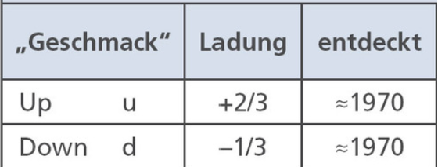
\includegraphics[scale=1]{bilder/pdf/quark_tabelle.pdf}
	%	\caption{Tabelle Ladung von Quarks}
%	\end{center}
%\end{figure}

\begin{table}[ht]
	\centering
	\renewcommand{\arraystretch}{1.5} % Zeilenhöhe anpassen
	\begin{tabular}{>{\centering\arraybackslash}m{3cm}|>{\centering\arraybackslash}m{3cm}}
		\multicolumn{2}{c}{\textit{\textbf{Quark Tabelle}}} \\
		\hline
		\textbf{Art} & \textbf{Ladung} \\
		\hline
		Up \( u \) & \( + \frac{2}{3}e \) \\
		Down \( d \) & \( - \frac{1}{3}e \) \\
		\hline
	\end{tabular}
	\caption{Up-Down-Quark Ladungen}
	\label{tab:quark_tabelle}
\end{table}

\section[Historische Methoden]{Historische Methoden zur Bestimmung der Elementarladung}\label{sec:historischeMethoden}
In dieser Arbeit steht der Millikan-Versuch zur Bestimmung der Elementarladung im Fokus. Dennoch sind auch andere Methoden erwähnenswert, wie beispielsweise das Experiment von Joseph John Thomson oder die Elektrolyse.

\subsection{Thomsonsche Methode}\label{sub:thomson}
Das Thomson Experiment untersucht die Ablenkung eines Elektronenstrahls durch ein magnetisches Feld. Beim Durchqueren des Magnetfelds wird der Strahl aufgrund der Lorentzkraft abgelenkt. Thomson konnte durch die gezielte Variation der Stärke des Magnetfelds das Verhältnis von Ladung zu Masse ($\frac{e}{m}$) der Elektronen bestimmen.

Die direkte Bestimmung der Elementarladung war mit diesem Experiment jedoch nicht möglich. Erst später, als die Masse des Elektrons unabhängig ermittelt wurde, konnte über das von Thomson bestimmte Verhältnis indirekt auf die Ladung des Elektrons geschlossen werden.

\subsection{Elektrolyse}\label{sub:elektrolyse}
Eine weitere Methode zur Bestimmung der Elementarladung basiert auf der Elektrolyse. Bei der Elektrolyse wird eine elektrische Spannung angelegt, um chemische Reaktionen, wie die Zersetzung von Molekülen, in einer ionischen Lösung zu erzwingen. Durch die Messung der angelegten Spannung und der Anzahl der Ionen, die sich während des Prozesses bewegen, lässt sich die Elementarladung indirekt ermitteln.

Beide dieser Methoden – die Elektrolyse und das Thomson Experiment – ermöglichen eine indirekte Bestimmung der Elementarladung. Sie sind in diesem Kontext durchaus erwähnenswert. Allerdings erlaubt der Millikan-Versuch eine wesentlich direktere Messung der Ladung kleinster Teilchen, was ihn besonders hervorhebt.


\section{Theorie des Versuchs}\label{sec:versuchsTheorie}
Da die anderen Methoden nur kurz behandelt wurden, wird der Millikan-Versuch nun detaillierter erklärt, zumindest in Bezug auf die zugrunde liegende Theorie.\\

\noindent Der Millikan-Versuch beginnt mit der Beobachtung eines Öltröpfchens im freien Fall. In \autoref{fig:freierFall} ist dieses Szenario schematisch dargestellt. Dabei wird die Bewegung des Tröpfchens durch die Gravitationskraft und die entgegengesetzt wirkende Reibungskraft bestimmt.

\begin{figure}[h]
	\begin{center}
		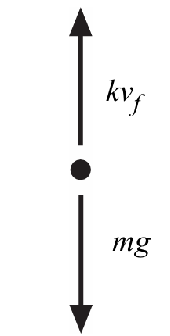
\includegraphics[scale=0.5]{bilder/pdf/Abbildung1_FreierFall.pdf}
		\caption{Öltröpfchen im Freien Fall \parencite[1]{instructionManualHalogen}}
		\label{fig:freierFall}
	\end{center}
\end{figure}

\noindent In Abbildung \ref{fig:freierFall} sind die Kräfte dargestellt, die auf ein Öltröpfchen im freien Fall wirken. Nach unten wirkt die Gewichtskraft, die proportional zur Masse des Tröpfchens $m$ und dem Ortsfaktor $g$ ist. Das Tröpfchen fällt durch die Luft und erreicht nach wenigen Millisekunden seine Endgeschwindigkeit $v_f$.

Die nach oben gerichtete Kraft ist die Reibungskraft der Luft, die von der Endgeschwindigkeit $v_f$ sowie dem Reibungskoeffizienten $k$ abhängt, welcher die Wechselwirkung zwischen der Luft und der Oberfläche des Tröpfchens beschreibt.

Im Zustand des Kräftegleichgewichts sind die beiden Kräfte, die Gewichtskraft und die Reibungskraft, exakt gleich gross, wodurch das Tröpfchen mit konstanter Endgeschwindigkeit fällt.

\begin{equation}\label{eq:kräfteFreierFall}
	mg \ = \ kv_f
\end{equation}   

\noindent Nun wird das Öltröpfchen in ein elektrisches Feld gesetzt. Mit den eingezeichneten Kraftvektoren sieht dies wie folgt aus:

\begin{figure}[h]
	\begin{center}
		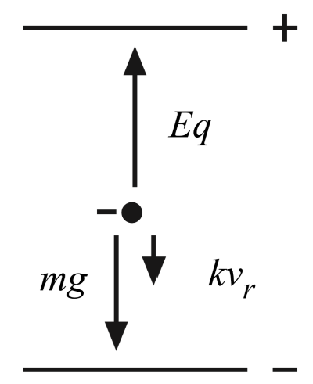
\includegraphics[scale=0.5]{bilder/pdf/Abbildung2_elektrischesFeld.pdf}
		\caption{Öltröpfchen im elektrischen Feld \parencite[1]{instructionManualHalogen}}
		\label{fig:elektrischesFeld}
	\end{center}
\end{figure}

\noindent Die elektrische Kraft, die in  Gleichung (\ref{fig:elektrischesFeld}) nach oben zeigt, ist abhängig von der elektrischen Feldstärke $E$ und der Ladung $q$ des Tröpfchens. Da die elektrische Kraft nun grösser als die Gewichtskraft ist, steigt das Tröpfchen. Wie oben im freien Fall behandelt, wirkt auch hier eine Reibungskraft der Luft, die entgegengesetzt der Bewegungsrichtung verläuft. Dieses Mal ist sie jedoch nicht von der Fallgeschwindigkeit abhängig, sondern von der Steiggeschwindigkeit $v_r$ (\textit{rise} auf Englisch: steigen) und, wie oben, vom Reibungskoeffizienten der Luft $k$.

Wenn man nun diese Vektoren algebraisch addiert, ergibt sich folgende Gleichung:

\begin{equation}\label{eq:elektrischesFeld}
	Eq \ = \ mg + kv_r
\end{equation}

\noindent Nun kann man nach $q$ umstellen und den Reibungskoeffizienten $k$ mithilfe von Gleichung (\ref{eq:kräfteFreierFall}) eliminieren. 

\begin{equation}\label{eq:hauptgleichung}
	q \ = \ \frac{mg \cdot (v_f + v_r)}{Ev_f}
\end{equation}

\noindent Die Masse eines Öltröpfchens zu bestimmen, ist in diesem Fall nahezu unmöglich. Aus diesem Grund versucht man, über die Dichte des Öls $\rho$ und das Volumen der Ölkugel auf die Masse zu schliessen. Der Zusammenhang zwischen Dichte und Masse lautet: $\rho \ = \ \frac{m}{V} \ \Leftrightarrow \ m \ = \ \rho \cdot V$. Das Volumen kann nun mithilfe des Radius $a$ berechnet werden. Setzt man nun alles zusammen, kommt man auf folgende Formel für die Masse eines Öltröpfchens. 

\begin{equation}\label{eq:masseFormel}
	mg \ = \ \frac{4}{3} \pi a^3 \rho g
\end{equation}

\noindent Jetzt kann dieses $m$ mit dem $m$ in Gleichung (\ref{eq:hauptgleichung}) substituiert werden.

\begin{equation}\label{eq:ladungFormel}
	q \ = \ \frac{4\pi a^3\rho g (v_f + v_r)}{3(Ev_f)}
\end{equation}

\noindent Das neue Problem ist nun der Radius $a$. Die Tröpfchen sind zu klein, um den Radius direkt zu messen. Die Lösung des Problems findet sich im stokesschen Reibungsgesetz $(F_f \ = \ 6\pi \eta a v_f)$, das den Zusammenhang zwischen Fallgeschwindigkeit und Reibungskraft der Luft beschreibt. Diese Formel beschreibt, wie sich ein kugelförmiges Objekt in einem viskosen Medium verhält. Das Gesetz hängt von der Viskosität der Luft $\eta$ und der Fallgeschwindigkeit $v_f$ ab. Dieser Ausdruck kann mit dem rechten Ausdruck der Gleichung (\ref{eq:masseFormel}) gleichgesetzt werden. Wird nach $a$ aufgelöst, erhält man:

\begin{equation}\label{eq:stokesRadius}
	a \ = \ \sqrt{\frac{9\eta v_f}{2\rho g}}
\end{equation}

\noindent Das stokessche Reibungsgesetz ist leider inkorrekt, wenn die Fallgeschwindigkeit weniger als 0,1 cm/s beträgt. Da im Experiment Fallgeschwindigkeiten zwischen 0,01 und 0,001 cm/s (zwischen $10^{-4}$ und $10^{-6}$ m/s) gemessen werden, muss das Reibungsgesetz mit einem Korrekturfaktor multipliziert werden. Die effektive Viskosität ergibt sich aus:

\begin{equation}\label{eq:effViskosität}
	\eta_{eff} \ = \ \eta \left( \frac{1}{1 + \frac{b}{pa}} \right) 
\end{equation}

\noindent $b$ ist dabei eine Konstante und $p$ ist der atmosphärische Druck in Pascal. 

\noindent Nun wird $\eta_{eff}$ in Gleichung (\ref{eq:effViskosität}) für $\eta$ in Gleichung (\ref{eq:stokesRadius}) substituiert.

\begin{equation}\label{eq:korrekturRadius}
	a \ = \ \sqrt{\frac{9\eta v_f}{2\rho g} \left( \frac{1}{1 + \frac{b}{pa}}\right)}
\end{equation}

\noindent Gleichung (\ref{eq:effViskosität}) enthält den Radius $a$. Das Problem besteht darin, dass ein Term für $a$ gefunden wurde, der wiederum $a$ enthält. Der Ausdruck für $a$ in Gleichung (\ref{eq:korrekturRadius}) kann in eine quadratische Gleichung umgewandelt werden:

\begin{equation}\label{eq:quadraticRadius}
	\begin{split}
		a & \ = \ \sqrt{\frac{9\eta v_f}{2\rho g} \left( \frac{1}{1 + \frac{b}{pa}}\right)} \\
		a^2 & \ = \ \frac{9\eta v_f}{2\rho g} \left( \frac{1}{1 + \frac{b}{pa}}\right) \\
		a^2 + \frac{b}{p}a & \ = \ \frac{9\eta v_f}{2\rho g} \\
		a^2 + \frac{b}{p}a - \frac{9\eta v_f}{2\rho g} & \ = \ 0
	\end{split}
\end{equation} 

\noindent Jetzt wird Gleichung (\ref{eq:quadraticRadius}) nach $a$ aufgelöst:

\begin{equation}\label{eq:qRadius}
	a \ = \ \sqrt{\left( \frac{b}{2p}\right)^2 + \frac{9\eta v_f}{2\rho g}} - \frac{b}{2p}
\end{equation}

\noindent Es ist zu beachten, dass, im Gegensatz zu Gleichung (\ref{eq:korrekturRadius}), jetzt kein $a$ mehr im Ausdruck vorkommt. Nun wird der komplette Term für $a$ in Gleichung (\ref{eq:ladungFormel}) ersetzt.

\begin{equation}\label{eq:ladungMitEingesetzR}
	q \ = \ \frac{4\pi \left[ \sqrt{\left( \frac{b}{2p}\right)^2 + \frac{9\eta v_f}{2\rho g}} - \frac{b}{2p} \right]^3 \rho g(v_f + v_r) }{3(Ev_f)}
\end{equation}

\noindent Die elektrische Feldstärke $E$ kann auch wie folgt ausgedrückt werden:

\begin{equation}\label{eq:elektrischeFeldstärke}
	E \ = \ \frac{V}{d}
\end{equation}

\noindent Wenn jetzt $E$ aus Gleichung (\ref{eq:ladungMitEingesetzR}) mit $E$ aus Gleichung (\ref{eq:elektrischeFeldstärke}) ersetzt wird und die gesamte Gleichung weiter umgeformt wird, resultiert daraus:

\begin{equation}\label{eq:letzteFormel}
	q \ = \ \frac{4\pi}{3} \cdot \left[ \sqrt{\left( \frac{b}{2p}\right)^2 + \frac{9\eta v_f}{2\rho g}} - \frac{b}{2p} \right]^3 \cdot \frac{\rho gd(v_f + v_r)}{Vv_f}
\end{equation}




	

